\section{Lasso}
Lasso finder løsningen til optimerings problemet
\begin{align}
\min_{\beta_0, \beta} \cbr{\frac{1}{2n} \sum_{i=1}^n \del{y_i - \beta_0 - \sum_{j=1}^p x_{ij} \beta_j}^2}, \ \text{underlagt at } \sum_{j=1}^p \vert \beta_j \vert \leq t \label{eq:2.3}
\end{align}
Betingelsen $\sum_{j=1}^p \vert \beta_j \vert \leq t$ kan skrives mere kompakt ved $\Vert \beta \Vert_1 \leq t$.
Dette kan udtrykkes på matrix-vektor notation.
Lad \(\y=(y_1, \ldots, y_n)\) være en \(n\) dimensional vektor med responsvariable og \(\X\) være en $n \times p$ matrix med $x_i \in \R^p$ som den i'te række, da kan \eqref{eq:2.3} omskrives til
\begin{align*}
\min_{\beta_0, \beta} \cbr{\frac{1}{2n} \Vert \y - \beta_0 \mathbf{1} - \X \beta \Vert_2^2}, \ \text{underlagt at } \Vert \beta \Vert_1 \leq t,
\end{align*}
hvor \(\mathbf{1}\) er en \(n\) dimensionel vektor bestående af 1 og \(\Vert \cdot \Vert_2\) betegner den Euklidiske norm af vektorer.

Grænsen \(t\) begrænser summen af de absolutte værdier af parameter estimaterne.
Denne skal specificeres ved en ekstern procedure kaldet \textit{kryds validering}, som vil blive diskuteret i kap --.

Ofte standardiseres prediktorerne \(\X\) således at kolonnerne er centeret og har varians 1. Dvs \(\frac{1}{n} \sum_{i=1}^n x_{ij} = 0\) og \(\frac{1}{n} \sum_{i=1}^n x_{ij}^2=1\). Hvis ikke prediktorerne standardiseres da vil lasso estimaterne afhænge af enhederne.
Hvis prediktorerne er målt i samme enhed, da vil vi typisk ikke standardisere.
For fuldstændigheden, antager vi også at responsvariablen $y_i$ er centeret, dvs \(\frac{1}{n} \sum_{i=1}^n y_{i} = 0\).
Når data er centreret da kan vi se bort fra skæringen $\beta_0$ i lasso optimeringen.
Given en optimal lasso løsning \(\hat{\beta}\) på det centreret data, kan vi finde løsningen for det ikke-centreret data. Der gælder at
\begin{align*}
\hat{\beta}^{\text{ikke-centreret}} = \hat{\beta}^{\text{centreret}} \\
\hat{\beta}_0^{\text{ikke-centreret}} = \bar{y} - \sum_{j=1}^p \bar{x}_j \hat{\beta}_j
\end{align*}
Derfor ser vi bort fra skæringen resten af kapitlet.

Vi kan omskrive lasso problemet til Lagrange form
\begin{align}
\min_{\beta} \cbr{\frac{1}{2n} \Vert \y - \X \beta \Vert_2^2 + \lambda \Vert \beta \Vert_1} \label{eq:2.5}
\end{align}
for $\lambda \geq 0$.
Af Lagrange dualiteten er der en bijektion mellem \eqref{eq:2.3} og \eqref{eq:2.5}: for hver værdi af \(t\) hvor \(\Vert \beta \Vert_1 \leq t\) er opfyldt, da findes en tilhørende værdi af $\lambda$ som giver den samme løsning for \eqref{eq:2.5}.
Mens løsningen $\hat{\beta}_\lambda$ til \eqref{eq:2.5} løser grænse problemet med $t=\Vert \hat{\beta}_\lambda \Vert_1$

Variabel udvægelsen for ridge regression og lasso illustreres på figur \ref{fig:LassoRig}.
\begin{figure}[H]
\begin{minipage}{0.5\linewidth}
\scalebox{0.8}{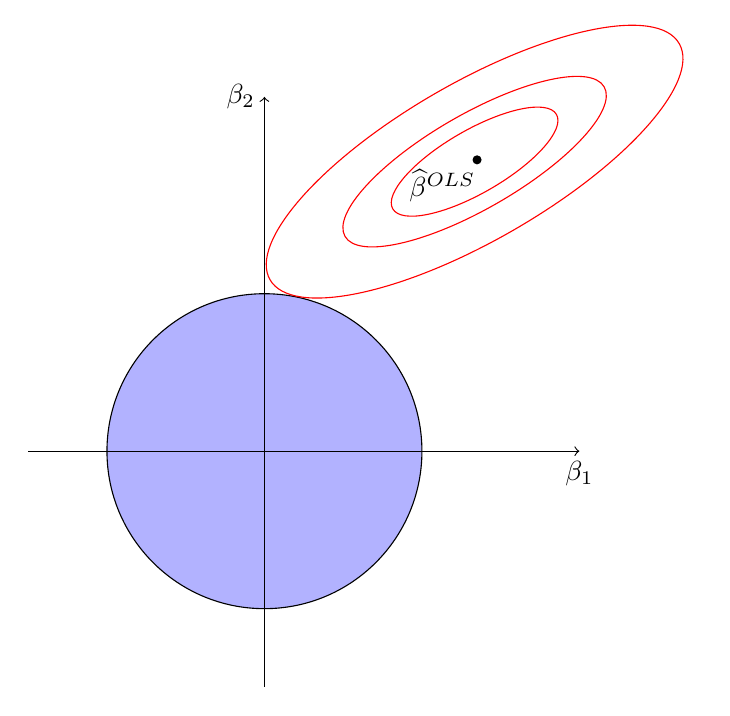
\begin{tikzpicture}
\draw [fill] (2.7,3.7) circle [radius=0.05];
\node [below left] (a) at (2.8,3.7) {$\widehat{\boldsymbol{\beta}}^\text{OLS}$};
\draw (0,0) circle (2cm) [fill= blue!30];
\draw [<-] (0,4.5) node [left] {$\beta_2$}-- (0,-3);
\draw[<-] (4,0) node [below] {$\beta_1$} -- (-3,0);
\begin{scope}[rotate = 30, red]
\clip[draw] (4.15,1.85) ellipse (3cm and 1cm);
\clip[draw] (4.15,1.85)ellipse (1.9 cm and 0.6 cm); 
\clip[draw] (4.15,1.85) ellipse (1.2 cm and 0.4 cm);
\end{scope}
\end{tikzpicture}}
\end{minipage}
\hspace{0.3cm}
\begin{minipage}{0.5\linewidth}
\scalebox{0.8}{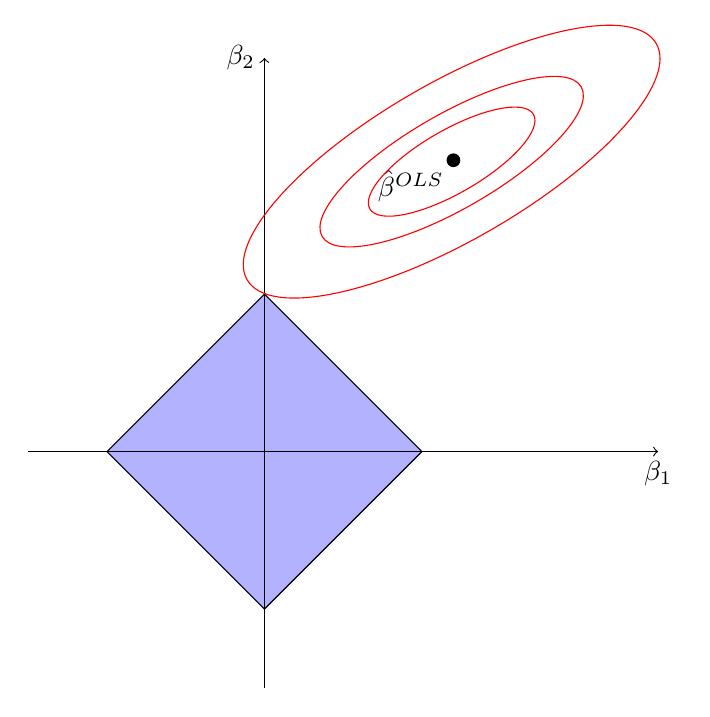
\begin{tikzpicture}
\draw [fill] (2.4,3.7) circle [radius=0.08];
\node [below left] (a) at (2.4,3.7) {$\hat{\beta}^\text{OLS}$};
\draw (-2,0) -- (0,2) -- (2,0)-- (0,-2) -- (-2,0)[fill = blue!30];
\draw [<-] (0,5) node [left] {$\beta_2$}-- (0,-3);
\draw[<-] (5,0) node [below] {$\beta_1$} -- (-3,0);
\begin{scope}[rotate = 30, red]
\clip[draw] (3.9,2) ellipse (3cm and 1cm);
\clip[draw] (3.9,2)ellipse (1.9 cm and 0.6 cm); 
\clip[draw] (3.9,2) ellipse (1.2 cm and 0.4 cm);
\end{scope}
\end{tikzpicture}}
\end{minipage}
\caption{Konturer for SSR og betingelsesområderne for ridge regression (venstre) og lasso (højre). De blå arealer er betingelsesområderne $\vert \beta_1 \vert+\vert \beta_2 \vert \leq t$ og $\beta_1^2+\beta_2^2 \leq t^2$, mens de røde ellipser er konturkurver for SSR. Konturkurverne har centrum i OLS estimatoren, $\hat{\beta}^\text{OLS}$.} \label{fig:LassoRig}
\end{figure}
For $p=2$ underligges OLS betingelsen $\beta_1^2 + \beta_2^2 \leq t^2$ for ridge regression og betingelsen $\vert \beta_1 \vert + \vert \beta_2 \vert \leq t$ for lasso.
Ellipserne omkring $\hat{\beta}^{\text{OLS}}$ er konturkurverne for SSR, dvs. SSR er konstant i en given ellipse. Værdien af SSR stiger, som ellipsen udvides fra $\hat{\beta}^{\text{OLS}}$.
Ligningerne - og - indikerer at løsningen for ridge regression og lasso er givet ved det første punkt, hvor konturkurverne rammer betingelsesområdet.
Siden ridge regression har et cirkulært betingelsesområde, vil skæringen med konturkurverne generelt ikke forekomme direkte på en akse.
Modsat ridge regression har lassos betingelses område hjørner i hver akse, hvilket betyder, at hvis løsningen forekommer i et hjørne, da vil en af parametrene $\beta_j$ være lig 0.

Hvis $t$ er tilstrækkelig stor, da vil betingelsesområderne indeholde $\hat{\beta}^{\text{OLS}}$ og derfor vil ridge regression og lasso estimatorerne være lig OLS estimatoren.

På figur \ref{fig:LassoRig} har vi blot betragtet det simple tilfælde hvor $p=2$. Når $p=3$ vil betingelsesområdet for ridge regression være en kugle, mens betingelsesområdet for lasso vil være en polydron. 

Da lasso penalty ikke er differentialbel, findes der ikke en eksplicit løsning til lasso problemet.
Vi antager at responsvariablerne $y_i$ og prediktorerne $x_{ij}$ er standardiseret således at \(\frac{1}{n} \sum_{i=1}^n y_{i} = 0\), \(\frac{1}{n} \sum_{i=1}^n x_{ij} = 0\) og \(\frac{1}{n} \sum_{i=1}^n x_{ij}^2=1\).
Da kan vi ser bort fra skæringen $\beta_0$.
Lagrange formen er nyttig for numerisk udregning af løsningen som findes vha en simpel procedure kaldet \textit{coordinate descent}.

Vi kan opskrive objektfunktionen i \eqref{eq:2.5} som
\begin{align*}
\frac{1}{2n} \sum_{i=1}^n \del{y_i - \sum_{k \neq j} x_{ik} \beta_k - x_{ij} \beta_j}^2 + \lambda \sum_{k \neq j} \vert \beta_k \vert + \lambda \vert \beta_j \vert
\end{align*}
Vi kan se at løsningen for hver $\beta_j$ kan udtrykkes ved den partial residual $r_i^{(j)}=y_i - \sum_{k \neq j} x_{ik} \hat{\beta}_k$, som fjerner ...
Da er den j'te koefficient opdateret ved
\begin{align}
\hat{\beta}_j = S_\lambda \del{\frac{1}{n} \left\langle \mathbf{x}_j, \mathbf{r}^{(j)} \right\rangle}, \label{eq:2.14}
\end{align}
hvor \(r_i = y_i - \sum_{j = 1}^p x_{ij} \hat{\beta}_j \) er de fulde residualer.
Den beskrevne algoritme svarer til metoden \textit{cyclical coordinate descent}, som minimerer en konveks objektfunktion langs hver koordinat af gangen.
Under milde regularitets betingelser, konvergerer løsningen til et global optimum.
Fra opdateringen \eqref{eq:2.14} ser vi at algoritmen foretager en univariat regression af den partial residual på hver prediktor, cycling gennem prediktorerne indtil konvergens.
\textit{pathwise coordinate descent}

Coordinate descent er særlig hurtig til at løse lasso problemet da ...

\textit{Homotopy metoder} er en alternativ teknisk til at løse lasso problemet. Disse producerer en helt sti af løsninger i en frekventiel sekvens, ved at starte med nul.
Denne sti er faktisk piecewise lineær.
Algoritmen kaldet \textit{least angle regression} (LARS) er en homotopy metode som effektivt konstruerer piecewise lineære stier.
En mere teoretisk gennemgang af coordinate descent og LARS algoritmen er givet i kapitel --. 
